\documentclass[%
fontsize=10%
,a5paper%
,DIV=15%
]{scrartcl}
%scrartcl



\usepackage{gredocument}
\usepackage{psaume}

\title{\centrer{Le Sacrement
de Baptême}}
\author{conféré aux adultes}
\date{}

\makeindex
\definecolor{rubrum}{rgb}{.6,0,0}
\def\rubrum{\color{rubrum}}%%%%%%%mettre"\def\rubrum{\color{rubrum}}" pour avoir le texte adéquat en rouge
\def\nigra{\color{black}}
%    \redlines
%    \definecolor{gregoriocolor}{rgb}{.6,0,0}
%
%\let\red\rubrum

\begin{document}


\maketitle

\newfontfamily\lettrines[Scale=1.3]{LettrinesPro800}
    \def\gretextformat#1{{\fontsize{\taillepolice}{\taillepolice}\selectfont #1}}
    \def\greinitialformat#1{{\lettrines #1}}

\titre{1. Au pied de l’autel}
\vspace{0.5cm}
\rubrica{1. Le prêtre, revêtu du surplis, de l’étole et de la chape violette, se rend au pied de l’autel avec ses ministres, et à genoux, demande humblement à Dieu d’être digne d’administrer un tel sacrement ; il implore l’aide divine, puis se relève, se signe et dit :}
\versio{V. Deus in adjutórium meum inténde.}{V. O Dieu, venez à mon aide.}
\versio{\textbf{R. Dómine ad adjuvándum me festína.}}{\textbf{R. Seigneur, hâtez-vous de me secourir.}

\rubrique{2. Puis il continue avec le clergé présent : }
\traduire{{\red {Ant.} Effúndam super vos aquam mundam, et mundabímini ab ómnibus inquinaméntis vestris, dicit Dóminus.}{{\red {Antienne}. Je répandrai sur vous une eau pure, et vous serez purifiés de toutes vos souillures, dit le Seigneur.}

\traduire{}{}


\titre{Les consentements}

\rubrica{Le prêtre s'adresse au fiancé :}

  \textsc{Mon{s}{i}eur {\rubrum{N.}}, voulez-vous prendre pour légitime épouse {\rubrum{N.}}, ici présente, selon le rite de notre mère la Sainte Eglise?}

\rubrique{Le fiancé répond : }  \textsc{Oui, je le veux.}

\rubrique{Puis, s'adressant à la fiancée :}

  \textsc{Mademoiselle {\rubrum{N.}}, voulez-vous prendre pour légitime époux {\rubrum{N.}}, ici présent, selon le rite de notre mère la Sainte Eglise?}

\rubrique{La fiancée répond : }  \textsc{Oui, je le veux.}

\rubrique{Le prêtre invite alors les époux à se donner la main droite. Puis il confirme l'engagement dont il vient d'être témoin en disant :}

\traduire{Ego conjungo vos in matrimonium, in nomine Patri, et Filii~\x\ et Spiritui Sancti. Amen.}{Je vous déclare unis par le mariage au nom du Père et du Fils~\x\ et du Saint Esprit. Ainsi soit-il.}

\vspace{0.5cm}
\titre{Bénédiction des Anneaux}

\rubrique{Le prêtre bénit les anneaux :}

\traduire{\V Adiutorium nostrum in nomine Domini.}{\V Notre secours est dans le nom du Seigneur.}

\traduire{\R \textbf{Qui fecit c\ae lum et terram.}}{\R \textbf{Qui a fait le ciel et la terre.}}


\traduire{%
\V~Dómine, exáudi oratiónem meam.}{%
\V~Seigneur, exaucez ma prière.}

\traduire{%
\R~\textbf{Et clamor meus ad te véniat.}}{%
\R~\textbf{Que mon appel vous parvienne.}}

\traduire{%
\V~Dóminus vobíscum.}{%
\V~Le Seigneur soit avec vous.}

\traduire{%
\R~\textbf{Et cum spíritu tuo.}}{%
\R~\textbf{Et avec votre esprit.}}

\traduire{%
Orémus.}{%
Prions.}

\traduire{ Bene~\x\ dic Domine annulum hunc quem nos in tuo nomine bene~\x\ dicimus, ut quæ eum gestaverit, fidelitatem integram suo sponso tenens, in pace et voluntate tua permaneat, atque in mutua caritate semper vivat.}{Béni~\x\ ssez, Seigneur, ces anneaux que nous béni~\x\ ssons en votre nom, afin que ceux qui les porteront, les conservent dans une fidélité entière, demeurent dans la paix et dans votre volonté, et qu'ils vivent toujours dans une mutuelle affection. Par le Christ Notre-Seigneur.}

\Amen

\rubrique{L'époux passe au doigt de son épouse et à son doigt l'anneau qui ne les quittera plus.
Le prêtre bénit ce geste et appelle les grâces divines sur l'union irrévocable qui vient de se conclure.}

\titre{Prière pour les époux}

\vspace*{0.5cm}
Au nom du Père~\x\ et du Fils et du Saint-Esprit. Ainsi soit-il.

\V Confirmez, Seigneur, ce que vous avez accompli en nous.

\R \textbf{De votre saint temple, en Jérusalem.}

Seigneur, ayez pitié de nous.
Christ, ayez pitié de nous.
Seigneur, ayez pitié de nous.

Notre Père... (à voix basse)

\V Et ne nous laissez pas succomber à la tentation. 

\R \textbf{Mais délivrez-nous du mal.}

\V Seigneur, sauvez vos serviteurs.

\R \textbf{Qui espèrent en vous, mon Dieu.}

\V Envoyez-leur votre aide, Seigneur, de votre sanctuaire.

\R\textbf{ Et de Sion, soutenez-les.}

\V Soyez pour eux, Seigneur, comme une tour fortifiée.

\R \textbf{Dressée contre l'ennemi.}

\V Seigneur, exaucez ma prière.

\R \textbf{Et que mon appel monte jusqu'à vous.}

\V Le Seigneur soit avec vous.

\R \textbf{Et avec votre esprit.}

Prions\\
Jetez les yeux, Seigneur, sur ces époux vos serviteurs et protégez cette institution que vous avez établie pour la propagation du genre humain, afin qu'unis par vous ils soient également soutenus et gardés par votre secours. Par le Christ Notre-Seigneur.

\R \textbf{Ainsi soit-il.}
\vspace*{3cm}
%\begin{center}
%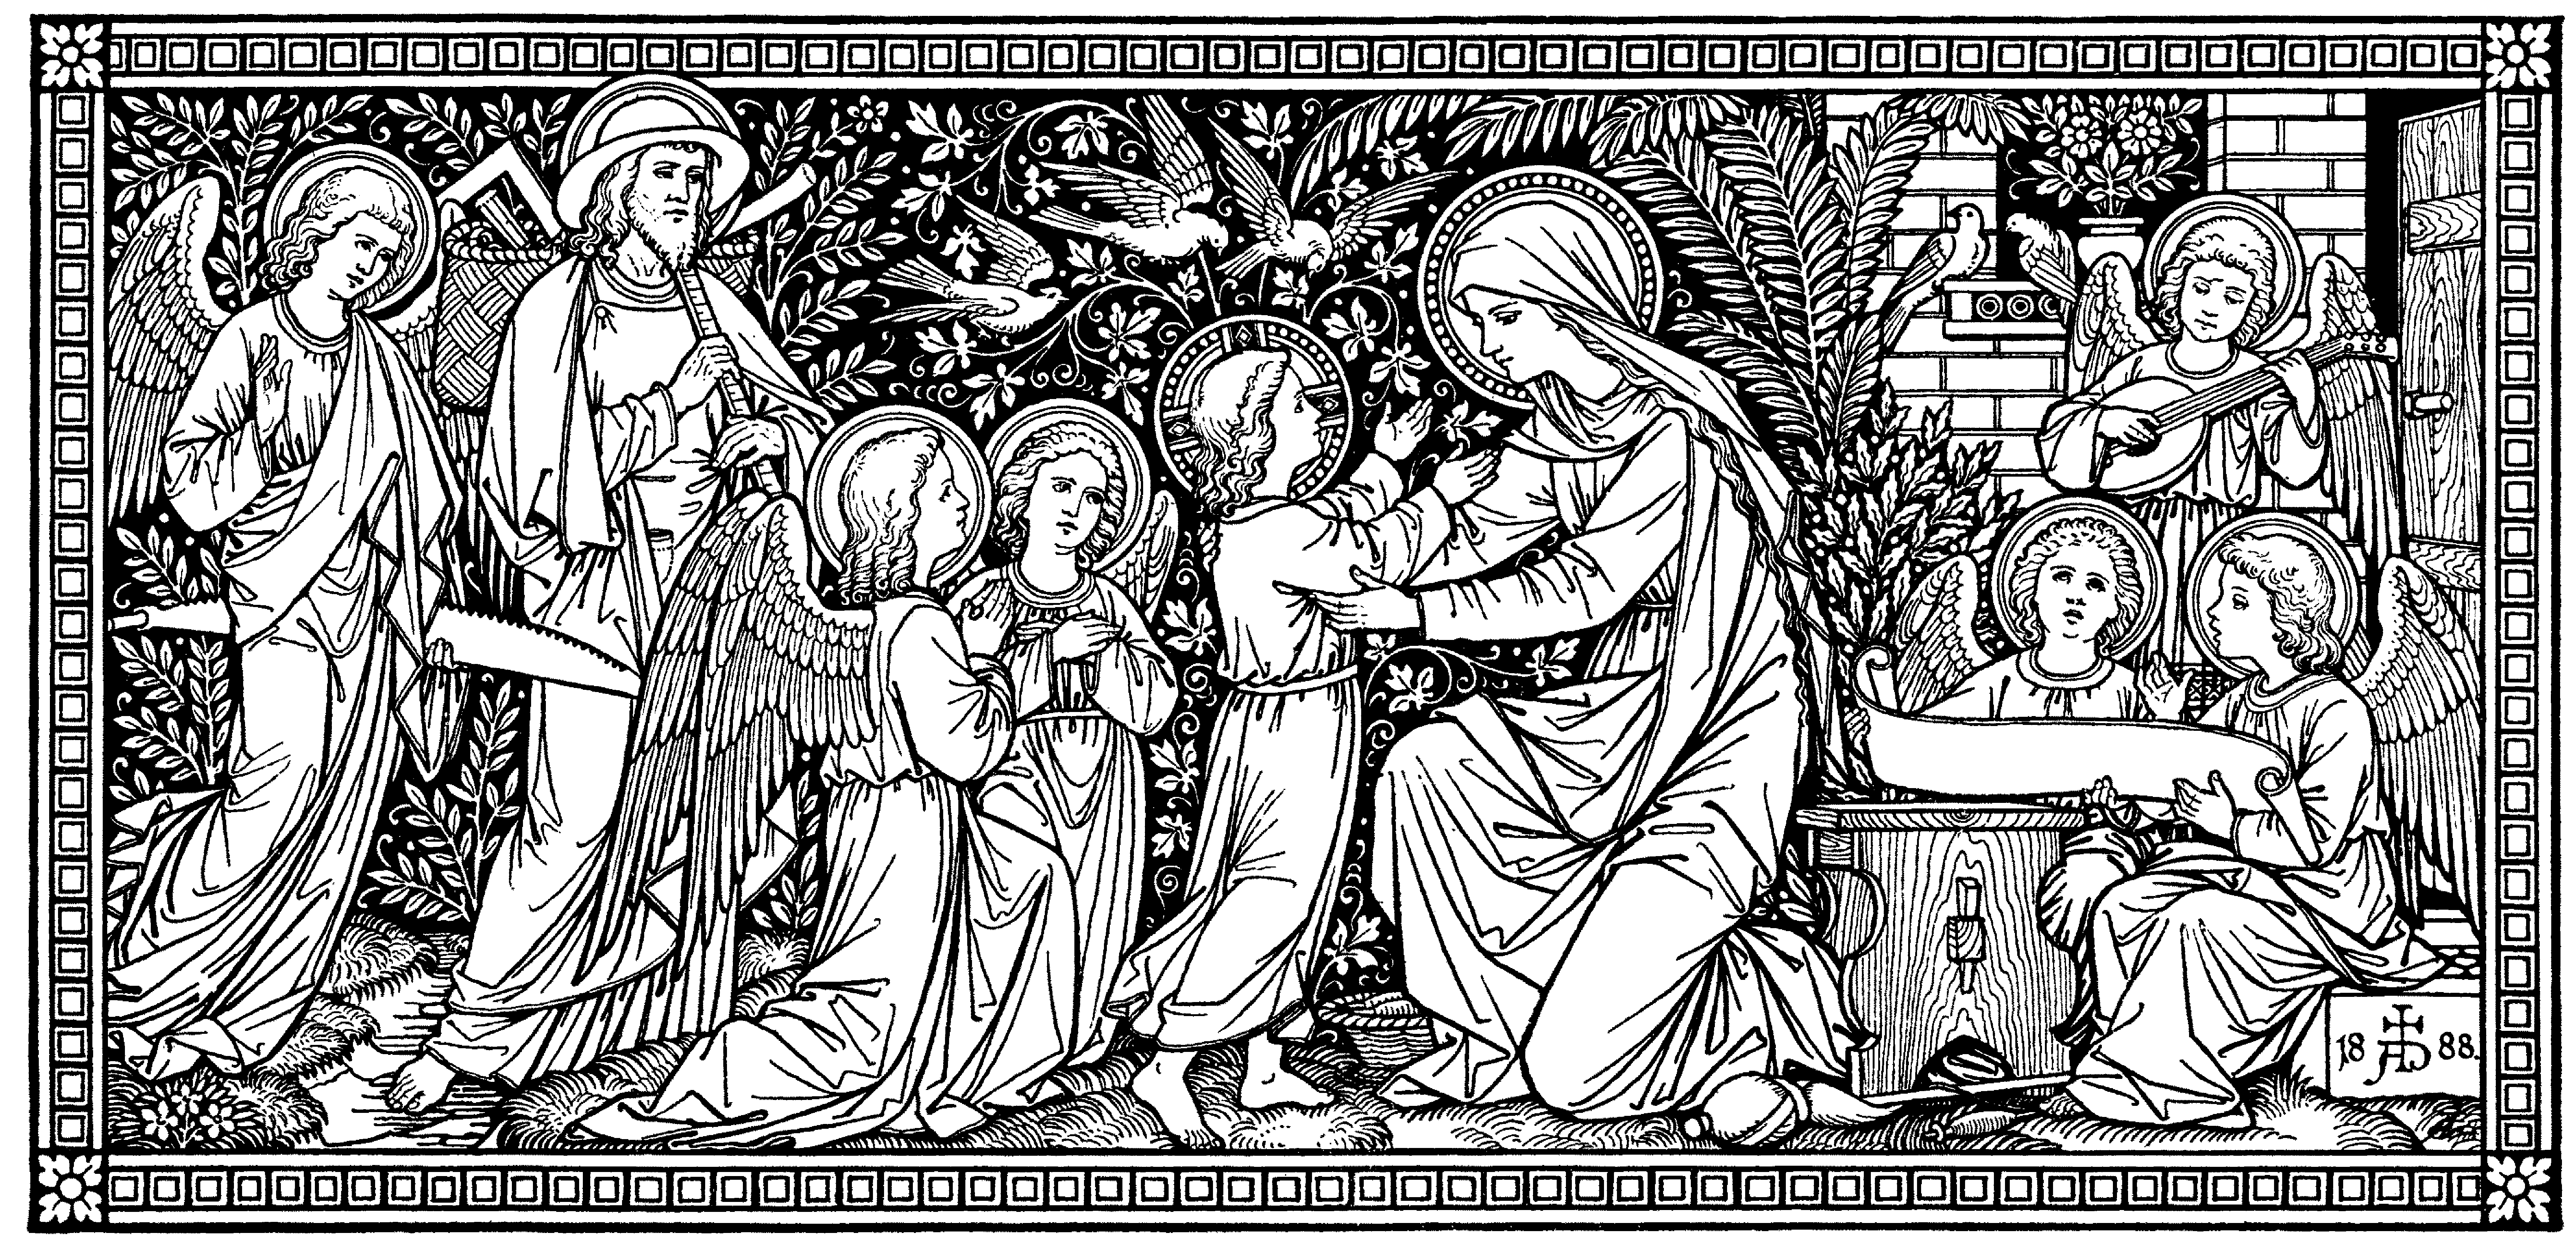
\includegraphics[height=5.5cm]{images/SainteFamille}
%\end{center}





\end{document}